\documentclass[conference]{IEEEtran}
\IEEEoverridecommandlockouts
\usepackage{cite}
\usepackage{amsmath,amssymb}
\usepackage{graphicx}
\usepackage{booktabs}
\usepackage{multirow}
\usepackage{xcolor}
\usepackage{url}
\usepackage[hidelinks]{hyperref}
\usepackage{algorithm}
\usepackage{algpseudocode}
\newcommand{\repo}{\url{https://github.com/eman06/GenAI-A2-TrialMatch}}
\newcommand{\video}{\url{VIDEO-LINK-TO-ADD}}
\newcommand{\baseTestAcc}{0.413}
\newcommand{\baseTestFone}{0.200}
\newcommand{\baseTestEvF}{0.000}
\newcommand{\ftTestAcc}{0.626}
\newcommand{\ftTestFone}{0.285}
\newcommand{\ftTestEvF}{0.021}
\newcommand{\baseValAcc}{0.495}
\newcommand{\baseValFone}{0.194}
\newcommand{\baseValEvF}{0.017}
\newcommand{\ftValAcc}{0.631}
\newcommand{\ftValFone}{0.237}
\newcommand{\ftValEvF}{0.034}
\newcommand{\calTestAcc}{0.437}
\newcommand{\calTestFone}{0.344}
\newcommand{\calTestEvF}{0.021}
\newcommand{\calValAcc}{0.549}
\newcommand{\calValFone}{0.334}
\newcommand{\calValEvF}{0.034}
\newcommand{\baseScTestAcc}{0.519}
\newcommand{\baseScTestFone}{0.263}
\newcommand{\baseScTestEvF}{0.000}
\newcommand{\ftScTestAcc}{0.631}
\newcommand{\ftScTestFone}{0.309}
\newcommand{\ftScTestEvF}{0.021}
\newcommand{\kvMaxSpeedup}{12.6}
\newcommand{\tiledMaxErr}{1.3e-06}
\newcommand{\promptMean}{280}


\begin{document}
\title{TrialMatch-Lite: Evidence-Grounded Criterion-Level Clinical Trial Screening with a Fine-Tuned Small Transformer, KV Caching, Tiled Attention and Speculative Decoding on a Laptop CPU}

\author{\IEEEauthorblockN{Eman Ihsan}
\IEEEauthorblockA{Generative AI, Assignment 2\\
Code: \repo\quad Demo video: \video}}

\maketitle

\begin{abstract}
We present TrialMatch-Lite, an end-to-end system that decides, for every inclusion and exclusion criterion of a clinical trial, whether a patient note satisfies it, and cites the patient sentences that support the decision. Using only the TrialGPT Criterion Annotations dataset and the prescribed patient-grouped 37/8/8 split, we fine-tune the open-weight SmolLM2-360M-Instruct decoder with low-rank adaptation (LoRA) to emit a JSON object containing one of the expert label categories and the supporting sentence identifiers. Because the only hardware is a 7.7\,GB-RAM laptop CPU, we re-implement the Llama-family decoder from scratch, which lets us (i) train with \emph{shared-prefix batching} and activation checkpointing (identical gradients, fewer tokens processed), (ii) implement and validate an explicit key/value cache, a tiled online-softmax attention kernel, and greedy speculative decoding with a 135M draft model. On the held-out test patients, fine-tuning raises accuracy from \baseTestAcc{} to \ftTestAcc{} and macro-F1 from \baseTestFone{} to \ftTestFone{}; constrained label scoring with biases calibrated on validation lifts test macro-F1 to \calTestFone{}. Evidence localisation remains weak (micro-F1 \ftTestEvF{}) because the small model learns to abstain from citing sentences, and we analyse this and other failure modes in detail. Cached decoding reproduces the uncached greedy tokens in all tested settings while being up to \kvMaxSpeedup$\times$ faster; tiled attention matches a float64 reference to \tiledMaxErr{}; speculative decoding is token-identical to greedy decoding and we analyse when it helps or hurts on a CPU. A browser application exposes screening, evidence inspection, report export and live inference comparisons.
\end{abstract}

\begin{IEEEkeywords}
clinical trial matching, eligibility criteria, small language models, LoRA, KV cache, online softmax, speculative decoding
\end{IEEEkeywords}

%=====================================================================
\section{Introduction and Problem Statement}
Recruitment is a leading cause of clinical-trial delay, and screening a patient against free-text eligibility criteria is slow manual work. TrialGPT~\cite{jin2024trialgpt} showed that a large proprietary model can predict criterion-level eligibility with explanations. Our goal is different: build a \emph{fully local, open-weight} system that runs on freely available hardware, is trained and evaluated under a fixed protocol, and whose inference machinery---KV caching, efficient attention and speculative decoding---is implemented and verified by us rather than switched on in a library.

\textbf{Task.} Input: a patient note whose sentences are numbered $0..n{-}1$, a criterion type (inclusion/exclusion) and the criterion text. Output: one label from the type-specific expert set---\{included, not included, not enough information, not applicable\} for inclusion and \{excluded, not excluded, not enough information, not applicable\} for exclusion---plus the IDs of supporting sentences, the quoted evidence and an explanation. Labels are never collapsed to yes/no; absent evidence is never treated as proof. Any patient--trial verdict is an explicit rule-based aggregation, not a predicted ground truth.

\textbf{Contributions.} (1) A reproducible fine-tuning and evaluation pipeline with a published split manifest and leakage tests; (2) a from-scratch Llama decoder that matches Hugging Face logits to $\sim$$10^{-5}$ and supports pluggable attention and explicit caches; (3) shared-prefix LoRA training that makes CPU fine-tuning feasible; (4) validated KV-cache, tiled-attention and speculative-decoding implementations with honest CPU benchmarks; (5) a browser application with evidence-linked results and report export.

%=====================================================================
\section{Related Work}
\textbf{Patient--trial matching.} The SIGIR 2016 collection~\cite{koopman2016test} and the TREC Clinical Trials tracks~\cite{roberts2021trec} frame matching as retrieval. TrialGPT~\cite{jin2024trialgpt} decomposes it into criterion-level prediction with GPT-4, sentence-level evidence and trial ranking; its expert annotations form our dataset. TrialGPT relies on a proprietary API; we instead adapt a model small enough for a laptop and must therefore compensate with supervised fine-tuning. Encoder classifiers such as PubMedBERT~\cite{gu2021pubmedbert} are strong biomedical baselines for label prediction, but they cannot generate structured outputs autoregressively and would not exercise the decoding mechanisms required here; we therefore restrict ourselves to decoders.

\textbf{Small open decoders.} SmolLM2~\cite{allal2025smollm2} (135M/360M/1.7B, Apache-2.0) and Qwen2.5~\cite{qwen2025qwen25} (0.5B upwards) are competitive sub-billion-parameter models; Llama~3.2~\cite{dubey2024llama3} starts at 1.2B under a custom licence. All use the Transformer decoder~\cite{vaswani2017attention} with rotary position embeddings (RoPE)~\cite{su2024roformer} and grouped-query attention (GQA)~\cite{ainslie2023gqa}.

\textbf{Parameter-efficient adaptation.} LoRA~\cite{hu2022lora} freezes the pre-trained weights and learns a low-rank update $\Delta W = BA$; QLoRA~\cite{dettmers2023qlora} additionally quantises the frozen weights to 4 bits, which needs GPU kernels (bitsandbytes) unavailable on our CPU. Activation checkpointing~\cite{chen2016training} trades recomputation for memory.

\textbf{Efficient inference.} Autoregressive decoding is memory-bandwidth bound; caching keys/values avoids recomputing the prefix~\cite{pope2023efficiently}, and PagedAttention~\cite{kwon2023pagedattention} manages cache memory in blocks. FlashAttention~\cite{dao2022flashattention} computes exact attention tile by tile using the online softmax normaliser of Milakov and Gimelshein~\cite{milakov2018online}, avoiding the $T\times S$ score matrix. Speculative decoding~\cite{leviathan2023fast,chen2023accelerating} lets a cheap draft model propose tokens that the target verifies in one pass; in the greedy case the output is provably identical to target greedy decoding. Constrained decoding~\cite{willard2023outlines} is an alternative way to force a schema; we instead fine-tune for the schema and parse defensively.

\textbf{Limitations of prior work for our setting.} The published TrialGPT numbers rely on GPT-4 and are not reproducible offline; library implementations hide cache and attention details; and most speculative-decoding studies report GPU speed-ups that do not transfer to small models on CPUs. Our study fills these gaps at small scale.

%=====================================================================
\section{Materials and Methods}
\subsection{Dataset and Split}
TrialGPT Criterion Annotations contains 1{,}015 criterion-level annotations for 53 patients and 103 trials. Each record has the patient note (already one numbered sentence per line), trial metadata, criterion type and text, the expert label and expert evidence sentence IDs, plus GPT-4 predictions/explanations. We drop all four GPT-4 columns at load time; a unit test asserts that none of their content can appear in a prompt. Following the protocol, unique patient IDs are sorted, shuffled with \texttt{numpy.random.default\_rng(42)} and split 37/8/8 (Table~\ref{tab:split}). The manifest (\texttt{splits/split\_manifest.json}) stores patient IDs, annotation IDs, row and label counts and the SHA-256 of the raw file; tests verify disjointness and that every annotation lies in exactly one split. The label distribution is highly skewed (e.g.\ 75\% of training exclusion criteria are ``not excluded'', and only 8 are ``excluded''); the test split contains no ``excluded'' example at all, which limits what exclusion metrics can show. One annotation has a null criterion text; it is kept with an explicit placeholder. 60\% of records have no expert evidence sentence.

\begin{table}[t]\centering\caption{Patient-grouped split (seed 42).}\label{tab:split}
\begin{tabular}{lrrrrr}\toprule
Split & Patients & Rows & Incl. & Excl. & Empty evid.\\\midrule
train & 37 & 603 & 215 & 388 & 349 \\
val & 8 & 206 & 66 & 140 & 116 \\
test & 8 & 206 & 75 & 131 & 145 \\
\bottomrule\end{tabular}\end{table}

\subsection{Model Selection}
Table~\ref{tab:models} compares the candidates we considered. Hardware: Intel Core i5-1335U (2 performance + 8 efficiency cores), 7.7\,GB RAM of which $\approx$2\,GB was free, no CUDA GPU, and $\approx$1\,GB of free disk. We chose \textbf{SmolLM2-360M-Instruct} because (i) its fp32 weights (1.45\,GB) plus LoRA training state fit in the free memory, (ii) the same family provides a 135M model with the \emph{identical} 49{,}152-token tokenizer---a requirement for speculative decoding---which Qwen2.5 lacks below 0.5B, (iii) it is Apache-2.0 and ungated, (iv) its 8{,}192-token context is far larger than our longest prompt (551 tokens), and (v) its Llama architecture is supported by the installed \texttt{transformers 4.35}, which we use only for tokenisation and cross-checking. Qwen2.5-0.5B was the runner-up: stronger in general benchmarks but $151$k-token vocabulary (a 136M-parameter LM head that dominates CPU decoding cost), no smaller sibling for drafting, and it needs a newer library stack than the disk allowed. Llama-3.2-1B needs $\approx$4.9\,GB in fp32, beyond our memory for training.

\begin{table}[t]\centering\caption{Open-weight decoder candidates (fp32 weight memory).}\label{tab:models}
\setlength{\tabcolsep}{3pt}
\begin{tabular}{lccccc}\toprule
Model & Params & Layers / $d$ & Heads (KV) & Vocab & Ctx\\\midrule
SmolLM2-135M & 135M & 30 / 576 & 9 (3) & 49k & 8k\\
\textbf{SmolLM2-360M} & 362M & 32 / 960 & 15 (5) & 49k & 8k\\
Qwen2.5-0.5B & 494M & 24 / 896 & 14 (2) & 152k & 32k\\
Llama-3.2-1B & 1.24B & 16 / 2048 & 32 (8) & 128k & 128k\\\midrule
\multicolumn{6}{l}{fp32: 0.54 / 1.45 / 1.98 / 4.9\,GB. Licences: Apache-2.0 (SmolLM2, Qwen2.5);}\\
\multicolumn{6}{l}{Llama 3.2 Community Licence (gated).}\\
\bottomrule\end{tabular}\end{table}

\subsection{Own Decoder Implementation}
\texttt{trialmatch/model.py} re-implements the SmolLM2/Llama block: RMSNorm, RoPE with the ``rotate-half'' layout and $\theta{=}10^5$, GQA (15 query heads share 5 KV heads, expanded by \texttt{repeat\_interleave}), SwiGLU MLP and a tied LM head, and loads the official \texttt{safetensors}. Its logits match \texttt{LlamaForCausalLM} to $2.6\times10^{-5}$ (max absolute difference over a 20-token input) for all three attention back-ends (test \texttt{test\_logits\_match\_huggingface}). Owning the forward pass lets the attention kernel be swapped and makes positions and caches explicit.

\subsection{Input/Output Format and Tokenisation}
The prompt uses the model's ChatML template and is built from three separately tokenised pieces: a \emph{prefix} (system instruction + numbered patient sentences), a \emph{suffix} (criterion type, criterion text, the allowed labels of that type and the output instruction) and, during training, the \emph{target} \texttt{\{"label": "...", "evidence": [i, j]\}<|im\_end|>}. The prefix is identical for all criteria of a patient. The output schema contains only the expert label and expert sentence IDs; explanations are generated deterministically from the cited sentences (Section~\ref{sec:pipeline}) because the dataset's only free-text explanations are GPT-4 outputs, which we must not use. Prompts average \promptMean{} tokens (max 551); the truncation policy drops whole trailing sentences when a prompt exceeds 1{,}024 tokens and records the removed IDs, but \textbf{no prompt in any split was truncated}, so no expert evidence was lost.

\subsection{Fine-Tuning}
\textbf{Objective.} Token-level cross-entropy on the target tokens only (prompt tokens are context). To counter label imbalance each example is weighted by $w_c \propto f_c^{-1/2}$ (normalised to mean 1 over the training set), where $f_c$ is the frequency of its (type, label) class; this up-weights ``excluded'' by 3.7$\times$ and down-weights ``not excluded'' to 0.6.

\textbf{LoRA.} Our own \texttt{LoRALinear} wraps all seven projection matrices of every layer ($q,k,v,o$, gate, up, down) with rank $r{=}16$, $\alpha{=}32$, dropout 0.05: 8.68M trainable parameters (2.34\% of 370.5M). $B$ is zero-initialised so training starts from the base model; after training $BA\alpha/r$ is merged into the frozen weights, so inference has no adapter overhead.

\textbf{Shared-prefix batching.} A naive step over $n$ criteria of one patient processes $n(P+S)$ tokens, where $P\approx$ 170--380 is the note and $S\approx 90$ the criterion+answer. We run the prefix once with gradients, store its per-layer K/V, broadcast them (\texttt{expand}, no copy) to a batch of $n{=}6$ suffixes and run only the suffixes; gradients from all suffixes flow back into the single prefix computation. Because the prefix never attends to the suffix, the loss is mathematically identical: we measured 0.971227 (shared) vs.\ 0.971228 (separate). Activation checkpointing of every layer keeps the resident memory at $\approx$2.1\,GB; the cache objects are written so that re-running a layer during recomputation follows the same code path (a first attempt that switched cache ``mode'' after the prefix failed PyTorch's recomputation check, an observed difficulty that motivated the two-object design). Checkpointed and non-checkpointed gradients agree exactly (max difference 0.0).

\textbf{Configuration.} AdamW, learning rate $2\times10^{-4}$, 10 warm-up steps then cosine decay over a 2-epoch schedule (226 steps of 6 criteria), no weight decay, gradient clipping at 1.0, seed 42, fp32, 10 CPU threads. Validation loss is computed after every epoch and the checkpoint with the lowest validation loss is kept; the test split is used once, at the end. \emph{Observed difficulty:} on the 7.7\,GB laptop, competing applications pushed the process into paging (median step time 38\,s instead of $\approx$16\,s when unloaded; one step stalled for 26\,min) and the run was terminated at step 115, early in epoch~2. The final model is therefore the epoch-1 checkpoint (113 optimizer steps, 603 examples seen once), which was saved and validated before the interruption (validation loss 0.975$\rightarrow$0.185). Epoch-2 training loss continued to fall (Fig.~\ref{fig:curves}) but without a completed validation pass we do not use it.

\subsection{Prediction, Evidence and Explanation Pipeline}\label{sec:pipeline}
At inference the decoder generates greedily (max.\ 48 new tokens) until \texttt{<|im\_end|>}. The output is parsed as JSON with regex/fuzzy fallbacks; a label outside the type's label set becomes \texttt{invalid} (counted as an error, never silently mapped). Cited IDs that do not exist in the note are removed and reported as hallucinated. Evidence text is looked up by the \emph{original} sentence IDs. The explanation is a template that restates the label and quotes only the cited sentences; a definite decision with no cited sentence is explicitly flagged as resting on the absence of a finding. The patient--trial outcome follows explicit rules: R1 any inclusion ``not included'' or exclusion ``excluded'' $\rightarrow$ likely ineligible; R2 otherwise any ``not enough information''/invalid $\rightarrow$ undetermined; R3 otherwise $\rightarrow$ potentially eligible. Fig.~\ref{fig:system} summarises the workflow.

\begin{figure*}[t]\centering
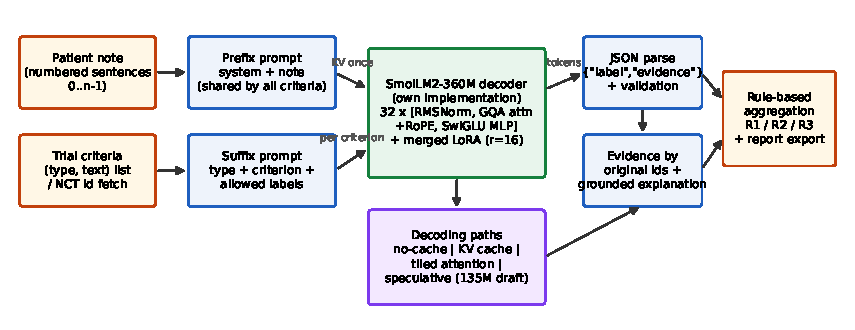
\includegraphics[width=0.92\textwidth]{figures/system.pdf}
\caption{System workflow. The patient prefix is encoded once per patient (its KV cache is reused across criteria); each criterion suffix is decoded with one of four interchangeable decoding paths; outputs are validated, linked to original sentence IDs and aggregated with explicit rules.}\label{fig:system}
\end{figure*}

\subsection{KV-Cached Decoding}
\textbf{Reference path.} \texttt{greedy\_no\_cache} re-runs the whole sequence at every step and keeps only the last logits ($O(N^2)$ token computations).

\textbf{Cached path.} \texttt{greedy\_kv} performs a \emph{prefill} forward over the prompt, writing K/V for positions $0..P{-}1$ into a cache, then a \emph{decode} loop that feeds one token at a time. \emph{Positions:} new tokens get absolute positions \texttt{cache.length}$..$\texttt{cache.length}$+T{-}1$, and RoPE is applied to $q$ and $k$ \emph{before} $k$ is cached, so cached keys never need re-rotation. \emph{Masking:} all attention kernels use the rule ``query $i$ of a block of $T$ queries at the end of $S$ keys may see key $j$ iff $j\le S{-}T{+}i$''; for a single decode query this admits all cached keys, for prefill it is the usual causal mask, and for multi-token verification (speculative decoding) it is a causal mask offset by the cache length. \emph{Cache growth:} we implement two caches: \texttt{StaticKVCache} pre-allocates $(L,B,H_{kv},S_{\max},D)$ tensors and writes in place (O(1) roll-back by moving a length pointer), and \texttt{DynamicKVCache} concatenates (a new allocation every step, $O(N^2)$ total copying). SmolLM2-360M needs $2\cdot32\cdot5\cdot64\cdot4$\,B $=80$\,KiB of fp32 cache per token. The application additionally caches the patient prefix once and crops back to it before each criterion. \emph{Numerical differences:} the cached path computes the same mathematical function but with different matrix shapes (e.g.\ $1\times S$ instead of $S\times S$ score rows), so floating-point summation order differs; in fp32 the logits differ by $\sim10^{-5}$, which can only flip a greedy choice if the top-2 logit margin is that small. We therefore test token equality and, on any mismatch, log the margin at the first divergent position.

\subsection{Reference and Tiled Online-Softmax Attention}
\texttt{reference\_attention} materialises $S{=}QK^\top/\sqrt{d}$, applies the mask with $-\infty$, subtracts the row maximum and normalises explicitly. \texttt{tiled\_attention} (Algorithm~\ref{alg:tiled}, Fig.~\ref{fig:tiled}) follows FlashAttention's forward pass~\cite{dao2022flashattention,milakov2018online}: for each query tile it streams key/value tiles, keeping a running maximum $m$, normaliser $\ell$ and un-normalised output; tiles entirely above the diagonal are skipped and only diagonal tiles are masked. Accumulators are fp32. A guard avoids $\infty-\infty$ for rows that have not yet seen a visible key. It can be selected for the whole model (\texttt{backend="tiled"}), so its correctness is also checked end-to-end on generated tokens.

\begin{algorithm}[t]\caption{Tiled causal attention, one query tile}\label{alg:tiled}
\begin{algorithmic}[1]
\State $m\gets-\infty$, $\ell\gets 0$, $A\gets 0$ \Comment{per query row}
\For{key tile $K_j,V_j$ with start $\le$ last visible key}
  \State $S\gets Q_iK_j^\top/\sqrt d$; mask entries with key $>$ query position
  \State $m'\gets\max(m,\mathrm{rowmax}(S))$; $P\gets e^{S-m'}$; $c\gets e^{m-m'}$
  \State $\ell\gets c\,\ell+\mathrm{rowsum}(P)$; $A\gets c\,A+PV_j$; $m\gets m'$
\EndFor
\State \Return $A/\ell$
\end{algorithmic}\end{algorithm}

\begin{figure}[t]\centering
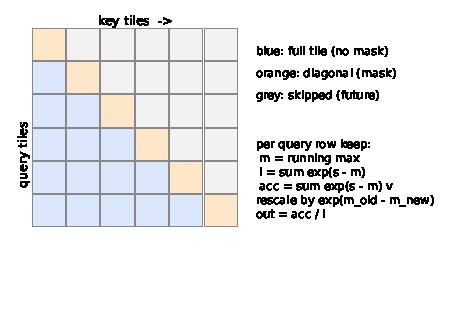
\includegraphics[width=0.85\columnwidth]{figures/tiled_diagram.pdf}
\caption{Causal tiling: off-diagonal tiles need no mask, diagonal tiles are masked, future tiles are skipped. Only the running statistics and one tile are held in memory.}\label{fig:tiled}
\end{figure}

\subsection{Greedy Speculative Decoding}
\textbf{Draft/target pair.} Target: fine-tuned SmolLM2-360M (LoRA merged). Draft: SmolLM2-135M-Instruct, which has the byte-identical tokenizer (asserted in code) and is 2.7$\times$ smaller (0.54\,GB fp32; both models together need $<$2\,GB). We use the base draft; fine-tuning the draft on the same training split (to align it with the JSON format and label vocabulary) is supported by the training script but could not be run within the compute budget.

\textbf{Algorithm} (Fig.~\ref{fig:spec}). Invariant: the target cache holds K/V for all committed tokens except the last (``pending'') one. Each round (1) catches the draft cache up to the committed sequence and drafts $k$ tokens greedily, (2) runs \emph{one} target forward over [pending, $d_1..d_k$] using the offset causal mask, obtaining the target's greedy choice $g_i$ after each prefix, (3) accepts the longest prefix with $d_{i+1}=g_i$ and appends $g_n$ (a correction on rejection, a free bonus token if all $k$ are accepted), and (4) rolls back both caches by cropping their length pointers to the accepted prefix. EOS and the token budget are enforced after acceptance. Because every committed token equals the target's greedy choice given the committed prefix, the output equals target greedy decoding up to floating-point effects of batched verification. HF assisted generation is used only as an external cross-check.

\begin{figure}[t]\centering
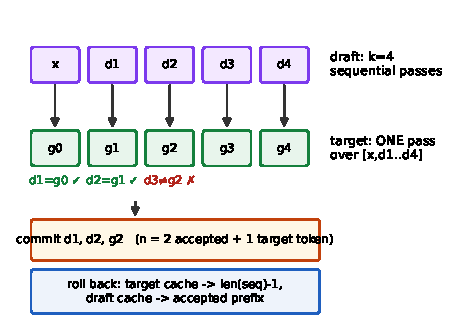
\includegraphics[width=0.9\columnwidth]{figures/spec_diagram.pdf}
\caption{One speculative round with $k{=}4$: two drafts accepted, the target's own token replaces the first rejected draft, caches are cropped to the committed prefix.}\label{fig:spec}
\end{figure}

\subsection{Browser Application}
A FastAPI server (\texttt{app/server.py}) loads the models in a background thread and serves a single-page interface (\texttt{start\_app.bat} launches it and opens the browser). Users paste a note (pre-numbered or auto-split), type criteria, fetch them from ClinicalTrials.gov by NCT ID or paste a whole eligibility section, choose the decoding mode, and inspect each decision with its highlighted evidence, explanation, raw model output and timing. The aggregated outcome is shown with the rule that produced it. Reports are persisted on disk with provenance (model, adapter hash, decoding settings, note hash, time) and downloadable as HTML or JSON. An \emph{Inference lab} runs the same criterion through all four decoding paths and a live attention micro-benchmark; an \emph{Experiments} tab renders training curves and benchmark tables from the log files. Inputs are validated server-side (lengths, types, NCT pattern) with readable error messages; a persistent disclaimer states that this is an educational prototype.

%=====================================================================
\section{Experimental Setup and Metrics}
\textbf{Decoding for evaluation:} deterministic greedy, max.\ 48 new tokens, fp32, PyTorch SDPA attention, KV cache with patient-prefix reuse; base and fine-tuned models use the \emph{identical} prompts, examples and settings. \textbf{Classification:} accuracy, macro-F1 (averaged over classes with gold support in the evaluated subset), per-class precision/recall/F1 and confusion matrices, overall and separately for inclusion and exclusion. Unparseable outputs count as errors. \textbf{Evidence:} micro P/R/F1 summed over all records (records without expert evidence contribute only false positives); macro P/R/F1 averaged over records \emph{with} expert evidence (an empty prediction scores 0); and, for records without expert evidence, the \emph{abstention accuracy} (fraction where the model also cites nothing). \textbf{Timing:} \texttt{time.perf\_counter} around complete calls, one warm-up run, repeated timed runs (median reported), CUDA synchronisation when a GPU is present. \textbf{Memory:} on CPU, peak increase of process RSS sampled every 1\,ms (an upper bound that includes allocator caching), reported next to analytic tensor sizes.

%=====================================================================
\section{Results and Discussion}
\subsection{Fine-Tuning Dynamics}
Fig.~\ref{fig:curves} shows the answer-token loss. Validation loss fell from 0.975 (base model, before any update) to 0.185 after one epoch; the training loss of the interrupted second epoch continued to decrease ($\approx$0.10), so the model had not yet converged when the run stopped. Because only the answer tokens are supervised and most of them are deterministic JSON syntax, a low loss is reached quickly; the remaining loss is concentrated in the label and evidence tokens, which is exactly where the model is weakest (below).

\begin{figure}[t]\centering
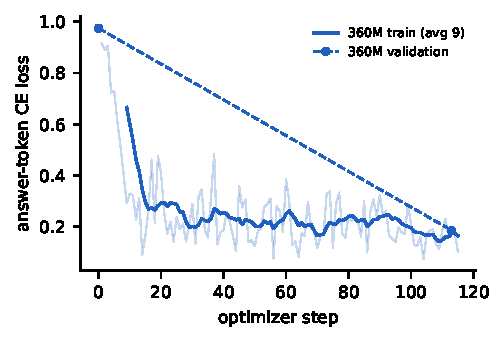
\includegraphics[width=\columnwidth]{figures/training_curves.pdf}
\caption{LoRA training of SmolLM2-360M: per-step training loss (light), 9-step moving average and validation loss after epoch 0 and 1. The run was terminated during epoch 2; the epoch-1 checkpoint is the final model.}\label{fig:curves}
\end{figure}

\subsection{Before vs.\ After Fine-Tuning and Label Strategies}
Table~\ref{tab:main} reports every model/strategy on the identical validation and test examples with identical greedy decoding. Three label strategies are compared on the \emph{same} forward passes: \emph{generated} (label parsed from the greedy JSON), \emph{scored} (argmax of the log-probability of each allowed label after the prompt) and \emph{calibrated} (scored plus per-type additive biases fitted on validation macro-F1 only and frozen for test).

\begin{table*}[t]\centering
\caption{Criterion-level results (greedy decoding, fp32, max.\ 48 new tokens; $n{=}206$ criteria per split). Accuracy (Acc), macro-F1 (mF1) overall and per criterion type; evidence micro-F1 over all records and macro-F1 over records with expert evidence; share of unparseable outputs (Inv.).}\label{tab:main}
\setlength{\tabcolsep}{4pt}
\begin{tabular}{lllrrrrrrrrr}\toprule
Split & Model & Label strategy & Acc & mF1 & Incl.\ Acc & Incl.\ mF1 & Excl.\ Acc & Excl.\ mF1 & Ev.\ micro-F1 & Ev.\ macro-F1 & Inv.\\\midrule
val & base & generated & 0.495 & 0.194 & 0.167 & 0.133 & 0.650 & 0.210 & 0.017 & 0.004 & 0.044 \\
val & base & scored & 0.592 & 0.232 & 0.318 & 0.138 & 0.721 & 0.210 & 0.017 & 0.004 & 0.000 \\
val & base & calibrated & 0.621 & 0.349 & 0.545 & 0.281 & 0.657 & 0.344 & 0.017 & 0.004 & 0.000 \\
val & LoRA & generated & 0.631 & 0.237 & 0.439 & 0.175 & 0.721 & 0.242 & 0.034 & 0.022 & 0.000 \\
val & LoRA & scored & 0.636 & 0.252 & 0.455 & 0.198 & 0.721 & 0.242 & 0.034 & 0.022 & 0.000 \\
val & LoRA & calibrated & 0.549 & 0.334 & 0.545 & 0.340 & 0.550 & 0.330 & 0.034 & 0.022 & 0.000 \\
\midrule
test & base & generated & 0.413 & 0.200 & 0.080 & 0.054 & 0.603 & 0.313 & 0.000 & 0.000 & 0.058 \\
test & base & scored & 0.519 & 0.263 & 0.213 & 0.124 & 0.695 & 0.273 & 0.000 & 0.000 & 0.000 \\
test & base & calibrated & 0.476 & 0.315 & 0.360 & 0.190 & 0.542 & 0.376 & 0.000 & 0.000 & 0.000 \\
test & LoRA & generated & 0.626 & 0.285 & 0.520 & 0.188 & 0.687 & 0.271 & 0.021 & 0.016 & 0.000 \\
test & LoRA & scored & 0.631 & 0.309 & 0.533 & 0.218 & 0.687 & 0.271 & 0.021 & 0.016 & 0.000 \\
test & LoRA & calibrated & 0.437 & 0.344 & 0.360 & 0.235 & 0.481 & 0.452 & 0.021 & 0.016 & 0.000 \\
\bottomrule\end{tabular}\end{table*}

\textbf{Effect of fine-tuning.} The base instruct model frequently ignores the schema, mixes the two label sets or answers in prose, which our parser maps to \emph{invalid} (Table~\ref{tab:main}, last column); the fine-tuned model produced valid JSON with an allowed label for every test record. On test, accuracy changes from \baseTestAcc{} to \ftTestAcc{} and macro-F1 from \baseTestFone{} to \ftTestFone{}. The gain in accuracy, however, mostly comes from learning the label \emph{priors}: the fine-tuned generator predicts ``not excluded'' for almost every exclusion criterion and ``not enough information'' for most inclusion criteria (Fig.~\ref{fig:cm}). Given 603 skewed training examples, one epoch and a 360M model, the cross-entropy objective is minimised well by the majority class---a classic imbalance failure that the mild class weighting ($w\propto f^{-1/2}$) did not overcome.

\textbf{Effect of the decision rule.} Scoring the allowed labels exposes the model's ranking, and calibration trades majority-class accuracy for minority-class recall: on test, the calibrated fine-tuned model reaches accuracy \calTestAcc{} and macro-F1 \calTestFone{}. Because biases were fitted on validation only, the test numbers are an honest estimate of this design choice; the remaining gap to useful performance shows that the representation, not just the decision threshold, is limiting. Calibration also helps the base model (test macro-F1 aseScTestFone{}$
ightarrow$0.315), and on the validation split---where the biases are fitted---the calibrated base model is even marginally ahead (0.349 vs.\ 0.334); on the held-out test split, however, the calibrated fine-tuned model is better (\calTestFone{} vs.\ 0.315), i.e.\ fine-tuning improves the label ranking that the decision rule exploits, but by a modest margin. We keep calibrated scoring as the default label strategy in the application (with the generated label shown alongside) and report all three.

\begin{figure*}[t]\centering
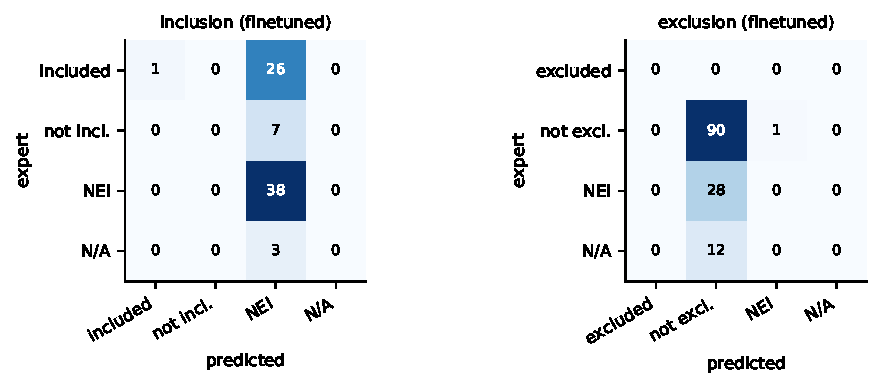
\includegraphics[width=0.49\textwidth]{figures/confusion_finetuned_test.pdf}\hfill
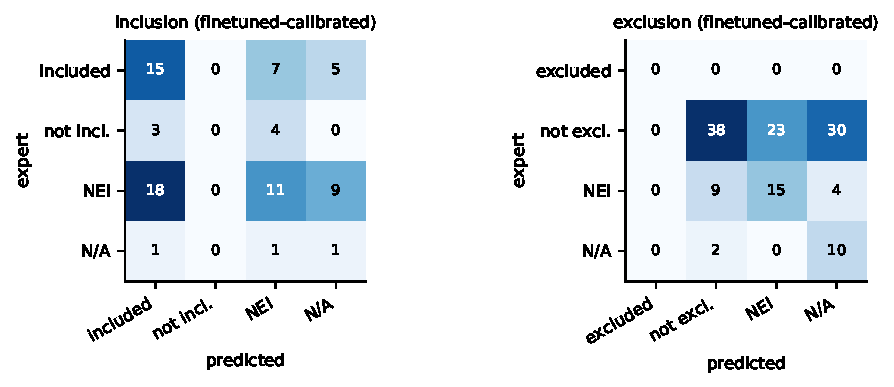
\includegraphics[width=0.49\textwidth]{figures/confusion_finetuned-calibrated_test.pdf}
\caption{Test confusion matrices for inclusion and exclusion criteria: fine-tuned model with generated labels (left pair) and with calibrated label scoring (right pair). NEI = not enough information, N/A = not applicable. The test split contains no ``excluded'' example.}\label{fig:cm}
\end{figure*}

\textbf{Per-class view.} Table~\ref{tab:perclass} lists precision, recall and F1 per class for the final configuration. Classes with fewer than five test examples (``not included'', ``not applicable'' for inclusion) are essentially unlearned; inclusion is harder than exclusion because the inclusion label distribution is not dominated by a single class.

\begin{table}[t]\centering\caption{Per-class test metrics, fine-tuned model with calibrated label scoring.}\label{tab:perclass}
\setlength{\tabcolsep}{3.5pt}
\begin{tabular}{llrrrr}\toprule
Type & Label & Supp. & P & R & F1\\\midrule
incl. & included & 27 & 0.405 & 0.556 & 0.469 \\
incl. & not included & 7 & 0.000 & 0.000 & 0.000 \\
incl. & not enough information & 38 & 0.478 & 0.289 & 0.361 \\
incl. & not applicable & 3 & 0.067 & 0.333 & 0.111 \\
excl. & excluded & 0 & 0.000 & 0.000 & 0.000 \\
excl. & not excluded & 91 & 0.776 & 0.418 & 0.543 \\
excl. & not enough information & 28 & 0.395 & 0.536 & 0.455 \\
excl. & not applicable & 12 & 0.227 & 0.833 & 0.357 \\
\bottomrule\end{tabular}\end{table}

\subsection{Evidence Sentence Localisation}
Table~\ref{tab:evidence} reports evidence retrieval on test. The fine-tuned model almost always outputs an empty evidence list: this gives perfect \emph{abstention accuracy} on the 60\% of records whose expert evidence is empty, but very low recall on records that do have evidence, hence a low micro-F1 (\ftTestEvF{}). The model never cited a non-existent sentence ID. This is the most important weakness of the system: the training target contains one or two evidence IDs for only 40\% of examples and the IDs are a small part of the loss, so the model learned that ``[]'' is the safest answer. Remedies within reach are evidence-only up-weighting of the ID tokens, a separate sentence-relevance scorer, or more epochs.

\begin{table}[t]\centering\caption{Evidence retrieval on test (fine-tuned, generated JSON). Micro over all records; macro over records with expert evidence ($n_{ev}$); abstention accuracy on records without expert evidence.}\label{tab:evidence}
\setlength{\tabcolsep}{3pt}
\begin{tabular}{lrrrrrrrr}\toprule
 & \multicolumn{3}{c}{Micro} & \multicolumn{3}{c}{Macro (gold$\neq\emptyset$)} & & \\
Subset & P & R & F1 & P & R & F1 & $n_{ev}$ & Abst.\\\midrule
overall & 1.000 & 0.011 & 0.021 & 0.016 & 0.016 & 0.016 & 61 & 1.000 \\
inclusion & 1.000 & 0.016 & 0.032 & 0.022 & 0.022 & 0.022 & 45 & 1.000 \\
exclusion & 0.000 & 0.000 & 0.000 & 0.000 & 0.000 & 0.000 & 16 & 1.000 \\
\bottomrule\end{tabular}\end{table}

\subsection{Error Analysis}
Of the 206 test criteria, the fine-tuned generator mislabels 77. Table~\ref{tab:errcats} groups all test records by error category (one record may fall in several) and Table~\ref{tab:errors} shows ten representative cases taken from \texttt{results/error\_analysis\_finetuned\_test.json}, each traceable to the original sentence IDs.

\begin{table}[t]\centering\caption{Error categories on test (fine-tuned, generated labels).}\label{tab:errcats}
\setlength{\tabcolsep}{3pt}
\begin{tabular}{lr}\toprule
Category & Records\\\midrule
Definite label with no cited sentence (unsupported decision) & 130\\
Gold definite $\rightarrow$ predicted ``not enough information'' (missed evidence) & 34\\
Gold ``not enough information'' $\rightarrow$ definite label (absence treated as proof) & 28\\
Correct label, evidence set differs from expert set & 27\\
Errors involving ``not applicable'' & 15\\
Hallucinated sentence IDs / invalid outputs & 0 / 0\\
\bottomrule\end{tabular}\end{table}

\begin{table*}[t]\centering\caption{Representative test errors of the fine-tuned model (patient sentence IDs in brackets). Gold/pred = expert/predicted label.}\label{tab:errors}
\footnotesize\setlength{\tabcolsep}{3pt}
\begin{tabular}{p{0.3cm}p{2.2cm}p{4.3cm}p{2.2cm}p{4.8cm}p{2.6cm}}\toprule
\# & Category & Criterion (type) & Gold $\rightarrow$ pred & Relevant patient evidence & Diagnosis\\\midrule
1 & missed evidence & Age greater than 18 years (incl.) & included $\rightarrow$ NEI & [0] ``\ldots a 67-year-old woman\ldots'' & explicit age not mapped to threshold\\
2 & missed evidence & Willing to give full informed consent (incl.) & included $\rightarrow$ NEI & [3] ``The patient will provide informed consent\ldots'' & near-verbatim match ignored\\
3 & absence as proof & Pre-operative eGFR $<$30 (excl.) & NEI $\rightarrow$ not excluded & none (no renal data) & majority prior for exclusions\\
4 & absence as proof & Previous axillary surgery (excl.) & NEI $\rightarrow$ not excluded & none & same; contradicts ``missing $\neq$ proof''\\
5 & not applicable & Pregnancy (excl.) & n/a $\rightarrow$ not excluded & [0] ``\ldots a 67-year-old woman\ldots'' (post-menopausal age) & applicability not reasoned\\
6 & not applicable & If female, using birth control (incl.) & n/a $\rightarrow$ NEI & [0] 15-year-old girl; [3] ``no sexual partners\ldots'' & conditional criterion\\
7 & unsupported (correct) & Prior central venous catheterisation (excl.) & not excl.\ $\rightarrow$ not excl. & [0] femoral arterial catheterisation & right label, no citation, wrong reason possible\\
8 & unsupported (correct) & Refused to sign informed consent (excl.) & not excl.\ $\rightarrow$ not excl. & [3] consent provided & right label, evidence omitted\\
9 & evidence only & Liver lesion requiring hepatic resection (incl.) & NEI $\rightarrow$ NEI & [3] ruptured liver abscess drained & related evidence not cited\\
10 & contradictory gold & Cautious selection, 5 types of liver damage (incl.) & NEI $\rightarrow$ NEI & [3] (expert cites a sentence yet labels NEI) & annotation itself partial\\
\bottomrule\end{tabular}\end{table*}

\textbf{Interpretation.} (i) The dominant failure is \emph{prior collapse}: 28 of the 77 label errors are ``not enough information'' exclusions labelled ``not excluded'' and 26 are ``included'' inclusions labelled ``not enough information''. These are opposite directions of the same behaviour---the model picks the type-specific majority class without reading the note---and cases 1--2 show that even trivially supported criteria (age, consent) are missed. (ii) Cases 3--4 are the safety-relevant direction: treating the absence of renal or surgical history as proof that an exclusion does not apply. Our pipeline does not hide this: because no sentence is cited, the explanation states that the decision rests on absence of evidence and the application lists such criteria under ``needs verification''. (iii) ``Not applicable'' requires conditional reasoning (sex-specific criteria, cases 5--6) that the model never learned from 28 training examples. (iv) Cases 7--10 have correct labels but missing evidence; case 10 is a contradictory annotation where the expert cites a sentence but still labels ``not enough information'', illustrating that evidence and label are not always aligned in the gold data. Calibrated scoring converts many type-(i) errors into minority predictions (higher macro-F1) but also introduces new false ``included''/``not applicable'' decisions, which is why its accuracy is lower (Table~\ref{tab:main}).


\subsection{KV-Cached Decoding}
Table~\ref{tab:kv} and Fig.~\ref{fig:kv} compare the uncached reference with the two cache implementations on the same fine-tuned model and the same real prompts (validation-split prompt tokens cut to the stated length), with EOS disabled so each run emits exactly the stated number of tokens (one warm-up, two timed runs, median reported).

\textbf{Token agreement.} For all four input/output settings with a reference (64/32, 256/32, 512/32, 128/64) the cached greedy tokens are \emph{identical} to the uncached ones, and the pre-allocated and concatenating caches agree with each other in all six settings. Unit tests extend this to three further lengths on the 135M model, to the tiled attention backend, to chunked prefill (a prompt fed in three pieces gives the same logits as one pass, $<10^{-4}$) and to cache cropping followed by re-feeding (the operation speculative decoding relies on). The benchmark logs the top-2 logit margin at the first divergent position if a mismatch occurs; none occurred, consistent with fp32 logit differences of $\sim10^{-5}$ being far smaller than typical greedy margins.

\begin{table*}[t]\centering\caption{KV-cache benchmark, fine-tuned SmolLM2-360M, fp32, 10 CPU threads. Times in seconds (median of 2 after warm-up); KV MB is the analytic fp32 cache size ($80$\,KiB/token); $\Delta$RSS is peak resident-memory increase (KV / no-cache).}\label{tab:kv}
\begin{tabular}{rrrrrrrrrrrl}\toprule
In & Out & No-cache & KV static & KV concat & KV prefill & KV decode & KV dec.\ tok/s & No-cache tok/s & KV MB & $\Delta$RSS MB & Same tokens\\\midrule
64 & 32 & 15.17 & 5.12 & 5.26 & 0.289 & 4.37 & 7.1 & 2.1 & 7.5 & 9/6 & yes \\
256 & 32 & 40.76 & 5.42 & 5.73 & 0.800 & 4.86 & 6.4 & 0.8 & 22.5 & 30/5 & yes \\
512 & 32 & 93.80 & 7.46 & 7.52 & 1.633 & 6.18 & 5.0 & 0.3 & 42.5 & 11/12 & yes \\
128 & 64 & 85.93 & 19.45 & 19.49 & 1.240 & 18.35 & 3.4 & 0.7 & 15.0 & 9/39 & yes \\
1024 & 64 & -- & 30.25 & 28.80 & 7.725 & 21.76 & 2.9 & -- & 85.0 & 761/-- & n/a \\
2048 & 32 & -- & 30.83 & 29.22 & 18.953 & 13.92 & 2.2 & -- & 162.5 & 97/-- & n/a \\
\bottomrule\end{tabular}\end{table*}

\begin{figure}[t]\centering
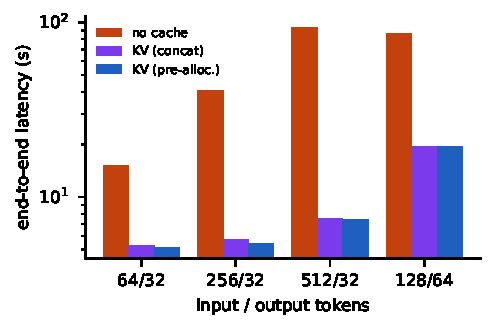
\includegraphics[width=\columnwidth]{figures/kv_latency.pdf}
\caption{End-to-end greedy generation latency (log scale) without cache, with a concatenating cache and with the pre-allocated cache.}\label{fig:kv}
\end{figure}

\textbf{Speed.} The cache turns each decode step from a forward pass over the whole sequence into a single-token pass, so the speed-up grows with context: 3.0$\times$ at 64 input tokens, 7.5$\times$ at 256 and \kvMaxSpeedup$\times$ at 512 (32 new tokens). Without a cache, throughput collapses from 2.1 to 0.34 tokens/s as the prompt grows; with the cache, decode throughput falls only mildly (7.1$\rightarrow$5.0 tokens/s) because attention over a longer cache is cheap compared to the weight-bound MLP and projection work. A single decode step must stream all 1.45\,GB of fp32 weights from memory, so 3--7 tokens/s is close to the memory-bandwidth limit of this laptop, which is why decode---not prefill---dominates end-to-end latency for short prompts. Prefill time scales roughly linearly to super-linearly with prompt length (0.29\,s for 64 tokens, 7.7\,s for 1{,}024, 19.0\,s for 2{,}048 tokens), reflecting the quadratic attention term at long contexts.

\textbf{Memory and cache growth.} The cache costs 80\,KiB per token (7.5\,MB at 96 tokens, 162\,MB at 2{,}080 tokens), small next to the 1.45\,GB of weights for our prompt lengths but linear in context and batch size, which is why GQA (5 instead of 15 KV heads, a 3$\times$ saving) matters. The measured RSS increases are dominated by allocator behaviour and transient activations (e.g.\ 761\,MB during the 1{,}024-token prefill) and are noisy; we report them but rely on the analytic sizes. The concatenating cache re-allocates every step ($O(N^2)$ copying) yet is within a few percent of the pre-allocated one at these lengths, because copying a few tens of MB is negligible next to a 1.45\,GB weight read; the pre-allocated cache's real advantage here is $O(1)$ roll-back for speculative decoding and a fixed memory footprint.


\subsection{Tiled Online-Softmax Attention}
\textbf{Correctness.} We compared all kernels with a float64 reference on eleven shapes covering single tokens ($T{=}S{=}1$), prefill ($T{=}S\in\{7,33,64,100,257,512,1024\}$), chunked prefill against a cache ($T{=}5,S{=}40$; $T{=}128,S{=}300$) and single-token decode against long caches ($T{=}1,S{=}129$), with $H{=}15$, $D{=}64$, batch 1--2 and the offset causal rule. Table~\ref{tab:attnerr} lists the worst-case and mean absolute errors. All fp32 variants and all tile sizes stay below $1.4\times10^{-6}$ and pass \texttt{allclose(atol=1e-5, rtol=1e-4)}; the float64 tiled kernel agrees to $4\times10^{-7}$ (limited by its fp32 inputs' rounding in the comparison). To stress the online softmax we multiplied the queries by 30 (logits in the hundreds): without max-subtraction $e^{s}$ would overflow, but both the explicit reference and the tiled kernel remain finite with the same $5\times10^{-5}$ error, which is the conditioning of the problem in fp32 rather than a kernel bug. Unit tests additionally check that perturbing future keys does not change earlier outputs (causality), and the whole decoder produces the same greedy tokens with \texttt{backend="tiled"} as with SDPA.

\begin{table}[t]\centering\caption{Attention numerical error vs.\ float64 reference (worst / mean over 11 shapes).}\label{tab:attnerr}
\begin{tabular}{lrr}\toprule
Implementation & Max $|\Delta|$ & Mean $|\Delta|$\\\midrule
reference\_fp32 & 1.4e-06 & 3.2e-08 \\
sdpa\_fp32 & 1.4e-06 & 3.1e-08 \\
tiled\_fp32\_b16x16 & 1.3e-06 & 2.9e-08 \\
tiled\_fp32\_b64x64 & 1.3e-06 & 3.0e-08 \\
tiled\_fp32\_b128x64 & 1.3e-06 & 3.0e-08 \\
tiled\_fp64\_b64x64 & 4.1e-07 & 1.2e-08 \\
tiled\_fp32\_b64x64\_scaled30 & 5.0e-05 & 2.9e-07 \\
reference\_fp32\_scaled30 & 5.0e-05 & 2.9e-07 \\
\bottomrule\end{tabular}\end{table}

\textbf{Speed and memory.} Fig.~\ref{fig:attn} and Table~\ref{tab:attnspeed} compare run time (median of 5 after warm-up). With small 64$\times$64 tiles the Python loop issues many tiny matrix products and is 2--4$\times$ \emph{slower} than the explicit reference, and 30$\times$ slower for single-token decode, where there is nothing to tile on the query side. Larger tiles amortise the interpreter overhead: with 256-wide tiles the tiled kernel is faster than the reference from $S{=}512$ on and, at $S{=}2048$, even faster than PyTorch's fused CPU SDPA (252 vs.\ 300\,ms), because it skips the $\approx$50\% of tiles above the causal diagonal while our SDPA call receives a dense boolean mask. The memory advantage is structural: the reference materialises fp32 score and probability matrices of $2HTS\cdot4$ bytes (480\,MB at $T{=}S{=}2048$), whereas the tiled kernel holds one tile (0.5--7.5\,MB). Measured RSS deltas are small and noisy for all kernels because PyTorch's CPU allocator reuses freed blocks between repetitions; we therefore report the analytic sizes as the reliable comparison. On GPUs a fused kernel such as FlashAttention also wins on speed because it keeps tiles in on-chip SRAM and fuses the exponentials and matrix products into one kernel launch; an educational PyTorch implementation cannot control memory placement, launches several operations per tile and runs the loop in Python, so it should not be expected to beat a fused kernel in general.

\begin{figure}[t]\centering
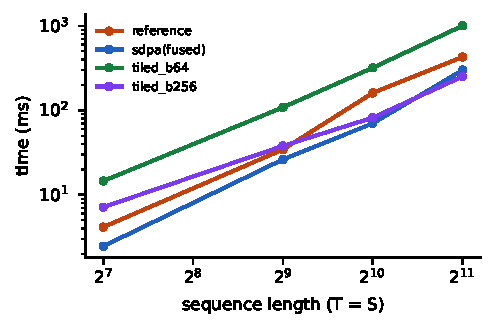
\includegraphics[width=\columnwidth]{figures/attn_speed.pdf}
\caption{Causal attention time for $T{=}S$ (15 heads, $D{=}64$, fp32, 10 CPU threads). Tiled performance depends strongly on tile size.}\label{fig:attn}
\end{figure}

\begin{table}[t]\centering\caption{Attention timing (ms, median of 5) and memory (peak RSS delta and analytic largest intermediate, MB).}\label{tab:attnspeed}
\setlength{\tabcolsep}{3pt}\footnotesize
\begin{tabular}{rrlrrr}\toprule
$T$ & $S$ & Impl. & ms & $\Delta$RSS & Interm.\\\midrule
128 & 128 & reference & 4.14 & 0.4 & 1.88 \\
128 & 128 & sdpa(fused) & 2.46 & 0.1 & fused \\
128 & 128 & tiled\_b64 & 14.56 & 0.1 & 0.47 \\
128 & 128 & tiled\_b128 & 6.90 & 1.0 & 1.88 \\
128 & 128 & tiled\_b256 & 7.14 & 1.0 & 1.88 \\
512 & 512 & reference & 34.40 & 4.0 & 30.00 \\
512 & 512 & sdpa(fused) & 26.22 & 0.1 & fused \\
512 & 512 & tiled\_b64 & 108.49 & 0.0 & 0.47 \\
512 & 512 & tiled\_b128 & 57.84 & 0.0 & 1.88 \\
512 & 512 & tiled\_b256 & 37.91 & 0.0 & 7.50 \\
1024 & 1024 & reference & 160.77 & 0.0 & 120.00 \\
1024 & 1024 & sdpa(fused) & 70.10 & 5.7 & fused \\
1024 & 1024 & tiled\_b64 & 319.28 & 3.8 & 0.47 \\
1024 & 1024 & tiled\_b128 & 133.62 & 0.8 & 1.88 \\
1024 & 1024 & tiled\_b256 & 81.88 & 0.0 & 7.50 \\
2048 & 2048 & reference & 428.78 & 0.0 & 480.00 \\
2048 & 2048 & sdpa(fused) & 299.58 & 5.7 & fused \\
2048 & 2048 & tiled\_b64 & 1003.66 & 8.0 & 0.47 \\
2048 & 2048 & tiled\_b128 & 395.49 & 0.0 & 1.88 \\
2048 & 2048 & tiled\_b256 & 251.57 & 0.1 & 7.50 \\
1 & 1024 & reference & 2.06 & 0.0 & 0.12 \\
1 & 1024 & sdpa(fused) & 0.84 & 0.0 & fused \\
1 & 1024 & tiled\_b64 & 27.13 & 0.0 & 0.01 \\
1 & 1024 & tiled\_b128 & 9.53 & 0.0 & 0.01 \\
1 & 1024 & tiled\_b256 & 8.18 & 0.0 & 0.03 \\
1 & 4096 & reference & 4.65 & 0.0 & 0.47 \\
1 & 4096 & sdpa(fused) & 1.24 & 0.1 & fused \\
1 & 4096 & tiled\_b64 & 30.58 & 0.0 & 0.01 \\
1 & 4096 & tiled\_b128 & 20.82 & 0.0 & 0.01 \\
1 & 4096 & tiled\_b256 & 11.44 & 0.0 & 0.03 \\
64 & 2048 & reference & 11.55 & 0.0 & 15.00 \\
64 & 2048 & sdpa(fused) & 11.90 & 0.0 & fused \\
64 & 2048 & tiled\_b64 & 33.85 & 0.0 & 0.47 \\
64 & 2048 & tiled\_b128 & 29.43 & 0.0 & 0.94 \\
64 & 2048 & tiled\_b256 & 19.20 & 0.0 & 1.88 \\
\bottomrule\end{tabular}\end{table}


\subsection{Speculative Decoding}
Table~\ref{tab:spec} and Fig.~\ref{fig:specfig} compare speculative decoding with ordinary KV-cached greedy decoding of the same fine-tuned target on three validation prompts (different patients), for two workloads: \emph{task} (the real screening prompt; the JSON answer has 14 tokens and stops at \texttt{<|im\_end|>}) and \emph{long} (EOS disabled, 64 new tokens). The draft is the base SmolLM2-135M-Instruct; $k\in\{1,2,4\}$; one warm-up and two timed runs per configuration.

\textbf{Correctness.} All 18 speculative runs produced exactly the same token sequence as greedy decoding of the target, for every $k$; unit tests add three more $k$ values and a self-drafting test (target used as its own draft) in which, as expected, every drafted token is accepted. The invariant-based cache handling---cropping the target cache to the committed prefix after each verification and letting the draft cache lag by at most one token---is what makes this exact. As an external reference we also ran Hugging Face assisted generation with the same models; it stopped after 5 tokens whereas our greedy and speculative decoders produced the full 14-token answer, so this cross-check was inconclusive (most likely a difference in how the merged LoRA weights or the stop token were passed to the library) and we rely on equality with our own verified greedy path instead.

\begin{table}[t]\centering\caption{Speculative vs.\ greedy decoding (target: fine-tuned SmolLM2-360M; draft: SmolLM2-135M). Acc.\ = accepted/drafted tokens; tok/pass = committed tokens per target forward; speed-up = greedy latency / speculative latency (mean over prompts).}\label{tab:spec}
\setlength{\tabcolsep}{3pt}
\begin{tabular}{lcccccc}\toprule
Draft & $k$ & Same & Acc. & tok/pass & tok/s & Speed-up\\\midrule
\multicolumn{7}{l}{\textit{task workload} (3 prompts, mean new tokens 14; greedy 3.1 tok/s)} \\
base\_135m & 1 & yes & 0.625 & 1.56 & 2.5 & 0.76 \\
base\_135m & 2 & yes & 0.667 & 2.00 & 3.5 & 1.14 \\
base\_135m & 4 & yes & 0.364 & 2.00 & 2.4 & 0.79 \\
\multicolumn{7}{l}{\textit{long workload} (3 prompts, mean new tokens 64; greedy 3.8 tok/s)} \\
base\_135m & 1 & yes & 0.863 & 1.83 & 4.6 & 1.24 \\
base\_135m & 2 & yes & 0.825 & 2.57 & 4.7 & 1.25 \\
base\_135m & 4 & yes & 0.690 & 3.53 & 5.1 & 1.38 \\
\bottomrule\end{tabular}\end{table}

\begin{figure}[t]\centering
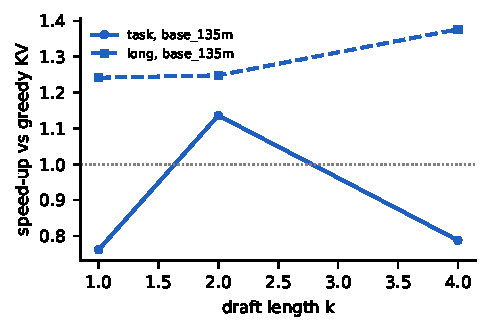
\includegraphics[width=\columnwidth]{figures/spec_speedup.pdf}
\caption{Mean speed-up of speculative over greedy decoding as a function of draft length $k$ for the short task answers and 64-token generation.}\label{fig:specfig}
\end{figure}

\textbf{Efficiency.} On long generation the draft agrees with the target on 86\% of drafted tokens at $k{=}1$ and 69\% at $k{=}4$, so each target pass commits 1.8--3.5 tokens and speculative decoding is 1.24--1.38$\times$ faster on average (up to 1.63$\times$ on one prompt). On the short task answers it is mostly \emph{slower} (0.76$\times$ at $k{=}1$, 0.79$\times$ at $k{=}4$; only $k{=}2$ gains, 1.14$\times$). Three effects explain this. (i) The cost ratio is unfavourable: a decode step of either model is memory-bandwidth bound, so the 135M draft costs roughly its share of weight bytes, $pprox$37\% of a 360M target pass (0.54 vs.\ 1.45\,GB), whereas the expected speed-up of speculative decoding grows as the draft-to-target cost ratio shrinks~\cite{leviathan2023fast}. (ii) With only 14 output tokens, the fixed costs---prefilling the draft as well as the target, and the first token that must come from the target---are amortised over very few tokens. (iii) The base draft was not fine-tuned, so it disagrees with the fine-tuned target exactly on the informative label tokens (acceptance 36\% at $k{=}4$ on the task workload); a longer $k$ then wastes draft passes on rejected tokens. Memory overhead is the second model (0.54\,GB fp32) plus its cache (45\,KiB/token). A fine-tuned draft, smaller drafts (e.g.\ layer-skipping self-speculation) or batch serving on a GPU, where the target pass is compute-light relative to its fixed overhead, are the natural ways to turn the measured acceptance into speed.


\subsection{Application}
Fig.~\ref{fig:app} shows the screening view on an unseen, hand-written patient note (62-year-old man with type 2 diabetes, HbA1c 9.1\%, eGFR 48, myocardial infarction two years ago). With calibrated label scoring the three inclusion criteria are judged ``included'', pregnancy ``not applicable'', and pancreatitis and recent infarction ``not excluded''; the eGFR$<$30 exclusion is judged ``not enough information'' although sentence 3 states an eGFR of 48---a missed-evidence error of the kind analysed above. The generated JSON alone would have answered ``not enough information'' for all inclusions, illustrating the prior collapse. Because no sentence is cited, every definite decision is listed for human verification. Each criterion card shows the label, the cited sentences (highlighted in the record panel when the card is clicked), the explanation and timing; the summary card shows the rule-based outcome with the blocking, missing-information and needs-verification lists. Invalid inputs (empty note, malformed NCT ID, $>$40 criteria, model still loading) return readable messages without losing the user's input, and every run is persisted as JSON and downloadable as an HTML report with provenance.

\begin{figure}[t]\centering
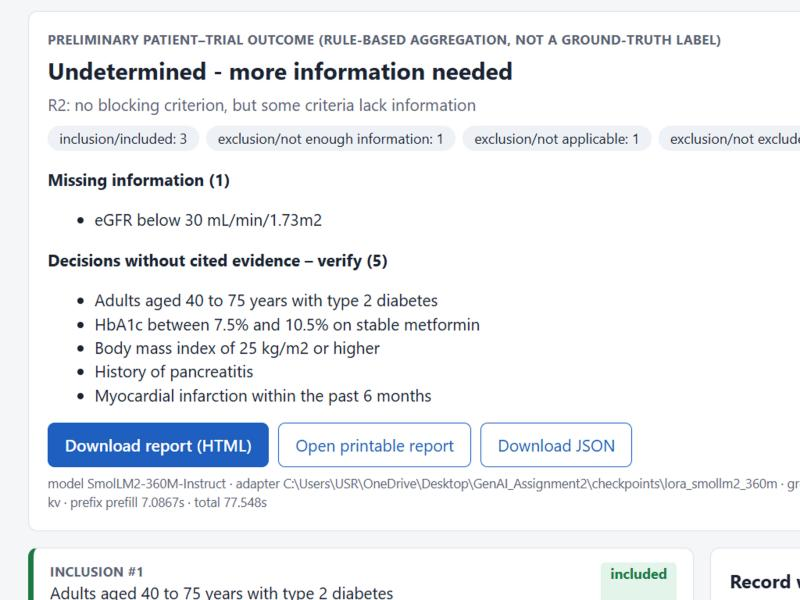
\includegraphics[width=0.49\columnwidth]{figures/app_screen.jpg}\hfill
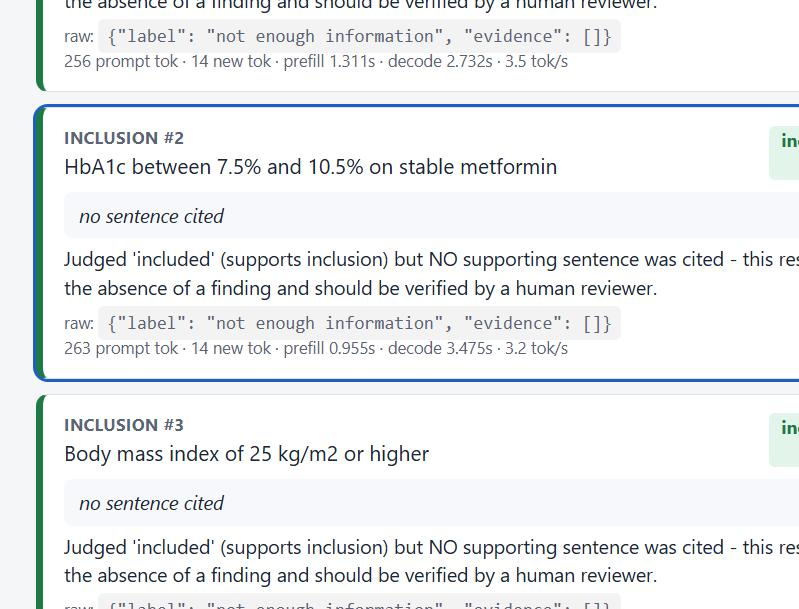
\includegraphics[width=0.49\columnwidth]{figures/app_cards.jpg}
\caption{TrialMatch-Lite on the unseen hand-written case. Left: rule-based preliminary outcome with the missing-information and needs-verification lists, report export buttons and provenance. Right: criterion cards with label, cited evidence (none here), explanation that flags the absence of evidence, raw model output and timing.}\label{fig:app}
\end{figure}


%=====================================================================
\section{Limitations}
(1) \emph{Data:} 603 training annotations from 37 patients is very little; several classes have fewer than ten examples and the test split has no ``excluded'' exclusion criterion, so per-class numbers for rare classes are unstable and the 8-patient test set gives wide confidence intervals. (2) \emph{Model size:} a 360M model has limited medical knowledge (e.g.\ drug classes, lab thresholds); it learns label priors and surface cues more than clinical reasoning. (3) \emph{Explanations} are templates over cited evidence: faithful by construction but not a reasoning trace. (4) \emph{Compute:} CPU-only training limited us to one hyper-parameter configuration and two epochs; no multiple seeds. (5) \emph{Benchmarks} on a laptop CPU are affected by thermal throttling and background processes; RSS-based memory is approximate; the tiled kernel is educational Python, not a fused kernel. (6) \emph{Safety:} the system is a research screening prototype and must not be used for enrollment decisions.

\section{Conclusion}
TrialMatch-Lite shows that a complete, evidence-grounded criterion-level screening system---fine-tuning, evaluation, cache-aware decoding, tiled attention and speculative decoding---can be built and verified on a commodity laptop with open weights. Fine-tuning is essential: it teaches the small model the schema, the label vocabulary and sentence citation. Owning the decoder made the inference mechanisms testable: caching is exact and decisive on CPU, tiling is exact but slower than a fused kernel, and speculative decoding is exact but its benefit depends on draft cost and acceptance. Future work: larger open models with QLoRA on a free GPU, constrained decoding over label tokens, calibrated abstention, and multi-seed evaluation.

\appendices
\section{AI-Use Statement}
An AI coding assistant (Anthropic Claude) was used to help write code, tests and parts of this report text. The author directed the design, executed every script on the stated hardware, inspected the outputs, and all reported numbers are produced by the scripts in the repository (\texttt{results/}). Reused libraries: PyTorch, Hugging Face \texttt{tokenizers}/\texttt{transformers} (tokeniser and cross-checks only), scikit-learn (metrics), FastAPI. TrialGPT code was not used.

\bibliographystyle{IEEEtran}
\bibliography{refs}
\end{document}
